\begin{frame}
  \frametitle{Récupération d'une architecture avec \emph{HWLOC}}
  \begin{figure}[t!]
    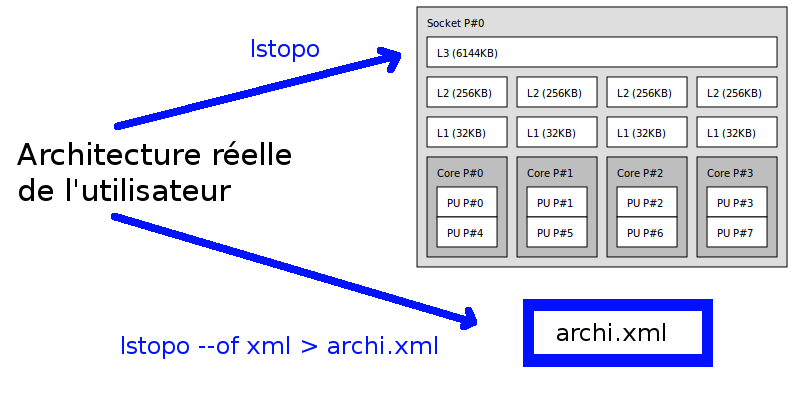
\includegraphics[width=.6\textwidth]{images/hwlocschema.png}
  \end{figure}

  Permet d'obtenir :
  \begin{itemize}
  \item Nom de l'architecture, du processeur
  \item Hiérachie entre les caches
  \item Pour chaque cache : taille, taille des lignes, associativité
  \end{itemize}

\end{frame}


\begin{frame}[fragile]
  \frametitle{Utilisation de \emph{HWLOC} pour \emph{Cassis}}

  Passage d'un fichier xml \emph{HWLOC} en entrée de \emph{Cassis} : création d'un fichier intermédiaire \\
\begin{verbatim}
  cassis -f archi.xml ...
\end{verbatim}

\begin{figure}[h!]
  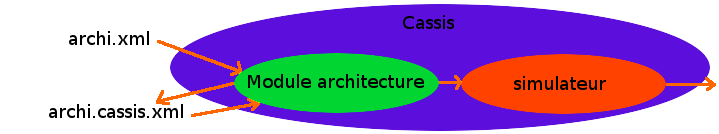
\includegraphics[width=.4\textwidth]{images/archicassis1.png}
\end{figure}

Passage d'un fichier xml \emph{Cassis} directement en entrée \\
\begin{verbatim}
  cassis -f archi.cassis.xml ...
\end{verbatim}

\begin{figure}[t!]
  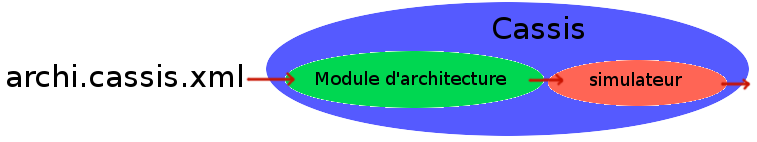
\includegraphics[width=.4\textwidth]{images/archicassis2.png}
\end{figure}
\end{frame}


\begin{frame}[fragile]
  \frametitle{Fichier d'architecture xml \emph{Cassis}}
  \begin{lstlisting}
  <?xml version="1.0"?>
  <Architecture name="x86_64" CPU_name="Intel(R) Core(TM) i5-3340M CPU @ 2.70GHz (modified)" number_levels="3">
      <Level depth="3" type="inclusive" directory_manager="false"/>
      <Level depth="2" coherence_protocol="MESI" type="nieo" snooping="true" directory_manager="false"/>
      <Level depth="1" coherence_protocol="MESI" snooping="true"/>
      <Cache depth="3" cache_size="3145728" cache_linesize="64" cache_associativity="12" replacement_protocol="LRU">
          <Cache depth="2" cache_size="262144" cache_linesize="64" cache_associativity="8" replacement_protocol="LRU">
              <Cache depth="1" cache_size="32768" cache_linesize="64" cache_associativity="8" replacement_protocol="LRU"/>
              <Cache depth="1" cache_size="32768" cache_linesize="64" cache_associativity="8" replacement_protocol="LRU"/>
          </Cache>
          <Cache depth="2" cache_size="262144" cache_linesize="64" cache_associativity="8" replacement_protocol="LRU">
              <Cache depth="1" cache_size="32768" cache_linesize="64" cache_associativity="8" replacement_protocol="LRU"/>
              <Cache depth="1" cache_size="32768" cache_linesize="64" cache_associativity="8" replacement_protocol="LRU"/>
          </Cache>
       </Cache>
   </Architecture>
  \end{lstlisting}
\end{frame}

\begin{frame}
  \frametitle{Paramètres non présents dans \emph{HWLOC}}
  \begin{itemize}
  \item<1-> Type d'inclusivité du cache \uncover<3->{{\color{blue}[L3 inclusif, L2 non inclusif]}}
  \item<1-> Protocole de cohérence \uncover<3->{{\color{blue}[MESI]}}
  \item<1-> Politique de remplacement \uncover<3->{{\color{blue}[LRU]}}
  \item<1-> Présence de \textit{snooping} dans un niveau de cache \uncover<3->{{\color{blue}[Oui]}}
  \item<1-> Présence d'un \textit{directory manager} \uncover<3->{{\color{blue}[Non]}}
  \end{itemize}
  \uncover<2->{Utilisation de {\color{blue} valeurs par défaut} (inspirées des architecture \emph{intel})}
\end{frame}

\begin{frame}
  \frametitle{\emph{Snooping} entre les caches}
  
\end{frame}


\begin{frame}
  \frametitle{Présence d'un \emph{directory manager}}
\begin{block}{Définition}
  \begin{itemize}
  \item Stocker les étiquettes des caches de niveau inférieur
  \item Connaître le contenu des descendants sans gaspiller trop d'espace mémoire (< 10\%)
  \end{itemize}
\end{block}

\begin{block}{Utilité}
\begin{itemize}
\item Chercher les données: par exemple pour le LLC dans le cas exclusif
\item Adadpter le remplacement des données pour les caches inclusifs, en évitant d'évincer des données présentes dans les caches descendants
\end{itemize}
\end{block}  
\end{frame}
